\documentclass[slidestop,compress,mathserif,red]{beamer}
\usetheme{Warsaw}
\usecolortheme{beaver}
\usepackage{hyperref}
\usepackage[utf8]{inputenc} % this is needed for german umlauts
\usepackage[english]{babel} % this is needed for german umlauts
\usepackage[T1]{fontenc}    % this is needed for correct output
                            % of umlauts in pd

\usepackage{graphicx}
\usepackage{caption}
\usepackage{fontspec}
\usepackage{xunicode}
\usepackage{xeCJK}
\setCJKmainfont[ItalicFont=Adobe Kaiti Std R, BoldFont=SimHei]{SimSun}
\setCJKsansfont{KaiTi}
\setCJKmonofont{SimHei}

  
\begin{document}

\title{进化树结构对比问题的算法研究}
\subtitle{Algorithm for Comparing Two Phylogenetic Trees}
\author{彭云}
\institute{指导老师:肖鸣宇}
\date{2015年3月11日}
\titlegraphic{
\includegraphics[width=0.2\textwidth, height=0.2\textheight, keepaspectratio]{./pic/logo.jpg}}

\frame{\titlepage}

\section{简介}
\begin{frame}{简介 - 进化树}
    进化树 (Phylogenetic tree):
    \begin{itemize}
      \item 是表明被认为具有共同祖先的各物种间演化关系的二叉树。
      \pause
      \item Example: \\
      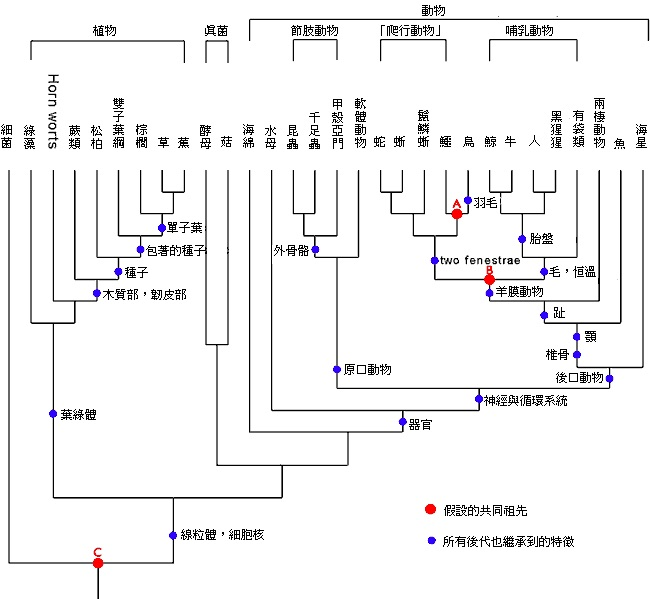
\includegraphics[width=0.5\textwidth, height=0.85\textheight, keepaspectratio]{./pic/Phylogenetic_tree_Chinese.jpg}
    \end{itemize}
\end{frame}

\begin{frame}{简介 - 网状事件}
    网状事件 (Reticulation events):
    \begin{itemize}
      \item 基因水平转移(horizontal gene transfer)
      \item 重组(recombination)
      \item 杂交(hybridization)
    \end{itemize}
\end{frame}

\begin{frame}{简介 - 杂交}
    杂交 (Hybridzation):
    \begin{itemize}
      \item 指不同种、属或品种的动、植物进行交配
      \pause
      \item Example: \\
      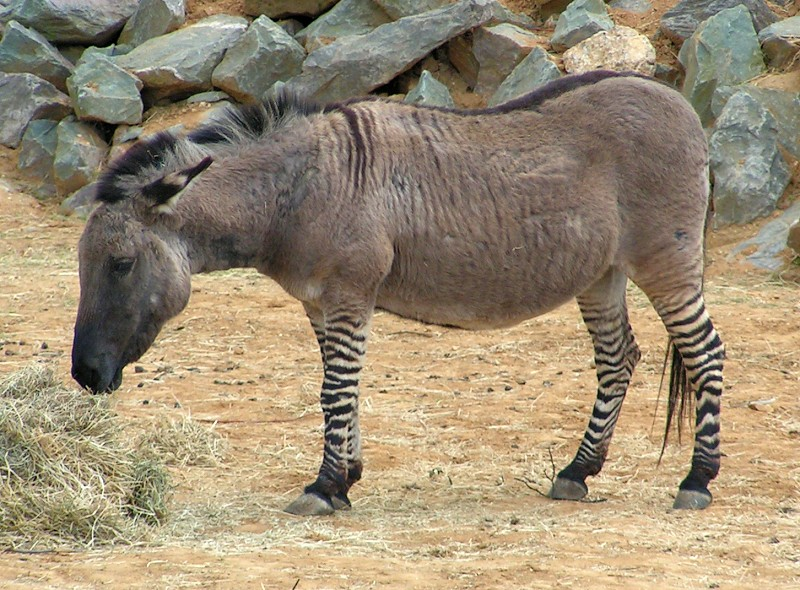
\includegraphics[width=0.35\textwidth, height=0.5\textheight, keepaspectratio]{./pic/zeedonk.jpg}
      \pause
      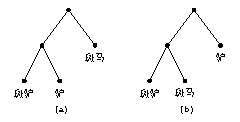
\includegraphics[width=0.65\textwidth]{./pic/3_animals.pdf}
    \end{itemize}
\end{frame}

\begin{frame}{简介 - rSPR distance}
    子树剪切再接距离(subtree prune and regraft distance, rSPR):
    \begin{itemize}
      \item 将二叉树的某棵子树剪下,再接到另外一条边上,收缩掉子节点个数为1的所有内部节点
      \pause
      \item Example: \\
      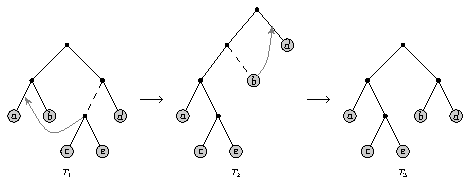
\includegraphics[width=0.9\textwidth, height=0.5\textheight, keepaspectratio]{./pic/tree_spr.pdf}
      \pause
      \item 将其中一棵树转化为另一棵所需的最少rSPR操作次数称为$T_1,T_2$的\textbf{rSPR距离},记作~$d(T_1,T_2)$
      \pause
      \item 难度:NP完全问题
    \end{itemize}
\end{frame}

\section{方法}
\begin{frame}{方法}
  \begin{itemize} 
    \item 固定参数算法(Fixed Parameter Algorithm):
    \begin{itemize}
      \item 给出一个参数k,通过搜索来判定两棵进化树之间的rSPR距离是否超过k
      \item 目前理论上最优的算法复杂度是$O(2.344^{k}n)$~~~\footnote{\tiny{Chen Z Z, Wang L. Faster exact algorithms for hybridization number and rSPR distance[J]. Submitted for, 2012.}}
      \newline{}
    \end{itemize}

    \pause

    \item 近似算法(Approximate Algorithm):
    \begin{itemize}
      \item 给出一个算法,使得这个算法的结果最差不会超过最优解的$r$倍
      \item 目前已经找到理论上最好的$r=3$的近似算法,复杂度为$O(n)$~~~ \footnote{\tiny{Whidden C, Zeh N. A unifying view on approximation and FPT of agreement forests[M]. Springer Berlin Heidelberg, 2009.}}
    \end{itemize}

    \pause

  \end{itemize}

  \begin{alertblock}{方向}
     主要研究基于固定参数算法的精确算法
     \newline{}
  \end{alertblock}
\end{frame}

\section{研究工具}

\begin{frame}{最大一致森林 - MAF}
    进化树森林:
    \begin{itemize}
      \item 将进化树$T$删去若干条边$E$,并对每棵子树进行收缩操作得到$F$,记作\textbf{$F=T-E$},同理有$F'=F-E$。
    \end{itemize}
    \pause
    最大一致森林(Maximum Agreement Forest):
    \begin{itemize}
      \item 若存在$E_1 \subset E_{T_1}$,$E_2 \subset E_{T_2}$,使得$F=T_1 - E_1$并且$F=T_2 - E_2$,我们称$F$为$T_1,T_2$的\textbf{一致森林}。
      \pause
      \item 将$T_1,T_2$包含最少进化树个数的森林称为\textbf{最大一致森林},其包含的进化树个数记为\textbf{$m(T_1,T_2)$}
      \pause
      \item Example: \\
      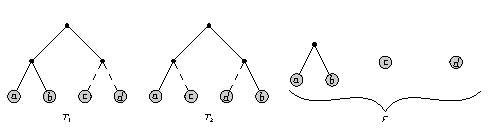
\includegraphics[width=0.9\textwidth, height=0.5\textheight, keepaspectratio]{./pic/maf.pdf}
      \pause
      \item $d(T_1,T_2) = m(T_1,T_2) - 1 $
    \end{itemize}
\end{frame}

\section{算法设计}
\begin{frame}{Whidden算法}
  在$T_1$中找一对兄弟叶节点,$F_2$中分三种情况:\\
  % \begin{itemize}
    % \item $ $\\
    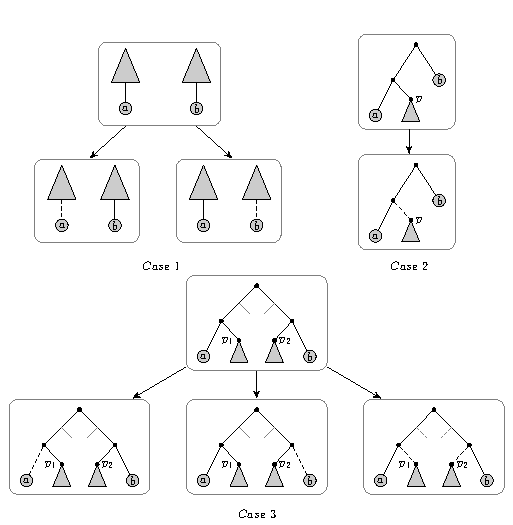
\includegraphics[width=0.9\textwidth, height=0.8\textheight, keepaspectratio]{./pic/3cases.pdf}
  % \end{itemize}
\end{frame}

\begin{frame}{Whidden算法复杂度}
\begin{itemize}
  \item 若$a,b$在$F_2$中属于不同的连通分量。
  \begin{equation*}
    C(k) \le 2C(k-1)
  \end{equation*}
  \item 若$a,b$在$F_2$中连通,并且$a,b$之间有且只有一个悬挂节点。
  \begin{equation*}
    C(k) \le C(k-1)
  \end{equation*}
  \item 若$a,b$在$F_2$中连通,并且$a,b$之间有至少两个悬挂节点。
  \begin{equation*}
    C(k) \le 2C(k-1) + C(k-m),~m \ge 2
  \end{equation*}
\end{itemize}
$C(k)$的最坏情况出现在第3种情况$m = 2$时,此时有
\begin{equation*}
C(k) \le 2C(k-1) + C(k-2)
\end{equation*}

设$C(k)=\alpha ^ k$,带入可得
\begin{equation*}
 1 = 2 \alpha ^ {-1} + \alpha ^ {-2}
\end{equation*}

得$\alpha = 1 + \sqrt{2} \approx 2.42$,复杂度为$O(2.42^kn)$
\end{frame}

\begin{frame}{改进方法}
    在$T_1$中找3个点或4个点
    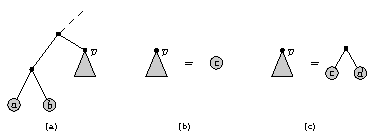
\includegraphics[width=0.9\textwidth, height=0.4\textheight, keepaspectratio]{./pic/3and4_pro.pdf}\\
    \pause
    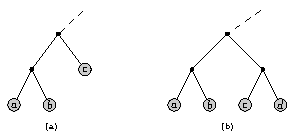
\includegraphics[width=0.9\textwidth, height=0.4\textheight, keepaspectratio]{./pic/3and4.pdf}
\end{frame}

\begin{frame}{三点情况}
\begin{itemize}
  \item Case 1.1:若$a,b$在$F_2$中属于不同的连通分量。
  \pause
  \item Case 1.2:若$a,b$在$F_2$中连通,且$|P(a,b)|=1$时。
  \pause
  \item Case 1.3:若$a,b$在$F_2$中连通,且$|P(a,b)| \ge 1$时。\\
  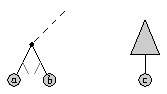
\includegraphics[width=0.9\textwidth, height=0.4\textheight, keepaspectratio]{./pic/case_1_3.pdf}
\end{itemize}
\end{frame}

\begin{frame}{三点情况}
Case 1.4:若$a,b$在$F_2$中属于相同的连通分量,满足$|P(a,b)| \ge 2$,且$a,b$与$c$属于同一连通分量
\pause
\begin{itemize}
  \item Case 1.4.1 若$a,c$或者$b,c$是兄弟节点。\\
  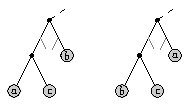
\includegraphics[width=0.9\textwidth, height=0.25\textheight, keepaspectratio]{./pic/case_1_4_1.pdf}
  \pause
  \item Case 1.4.2 若$F_2$中满足$|P(a,c)|=1$且$|P(b,c)|=1$ \\
  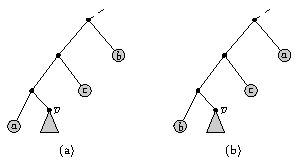
\includegraphics[width=0.45\textwidth, height=0.35\textheight, keepaspectratio]{./pic/case_1_4_2.pdf}
  ~~~
  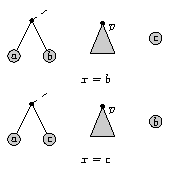
\includegraphics[width=0.45\textwidth, height=0.35\textheight, keepaspectratio]{./pic/case_1_4_2_eq.pdf}
\end{itemize}
\end{frame}

\begin{frame}{三点情况}
\begin{itemize}
  \item Case 1.4.3:  排除\textit{Case 1.4.1}和\textit{Case 1.4.2},$F_2$中一定有$|P(a,c)| \ge 1$且$|P(b,c)| \ge 1$且存在$x \in \{a,b\}$使$|P(x,c)| \ge 2$。不妨设$x=a$,综合之前的条件,有
        \begin{center}
        $\left\{
        \begin{array}{l}
          |P(a,b)| \ge 2\\
          |P(a,c)| \ge 2\\
          |P(b,c)| \ge 1
        \end{array}
        \right.$
        \end{center}

  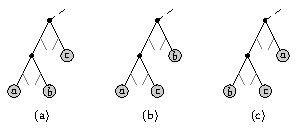
\includegraphics[width=0.9\textwidth, height=0.7\textheight, keepaspectratio]{./pic/case_1_4_3.pdf}

\end{itemize}
\end{frame}

\begin{frame}{四点情况}
  \begin{itemize}
    \item Case 2.1:若$a,b$(或$c,d$)在$F_2$中属于不同的连通分量
    \pause
    \item Case 2.2:若$a,b$(或$c,d$)在$F_2$中属于相同的连通分量,且$|P(a,b)|=1$(或$|P(c,d)|=1$)
    \pause
    \item Case 2.3:若$a,b$在$F_2$中连通,$c,d$也在$F_2$中连通,且满足$|P(a,b)| \ge 2,|P(c,d)| \ge 2$,但$a,b$与$c,d$不连通\\
    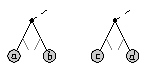
\includegraphics[width=0.4\textwidth, height=0.5\textheight, keepaspectratio]{./pic/case_2_3.pdf}
    \pause
    \item Case 2.4:若$a,b$在$F_2$中连通,$c,d$也在$F_2$中连通,且满足$|P(a,b)| \ge 2,|P(c,d)| \ge 2$,且$a,b,c,d$均连通\\
    
  \end{itemize}
\end{frame}

\begin{frame}{改进算法复杂度分析}
  \begin{center}
  $\left\{
  \begin{array}{l}
    C(k) \le 2C(k-1) ~~~~~~~~~~~~~~~~~~~~~~~~~~~~~~~~~~~ Cases~1.1,2.1\\
    C(k) \le C(k-1)  ~~~~~~~~~~~~~~~~~~~~~~~~~~~~~ Cases~1.2,1.4.1,2.2\\
    C(k) \le 3C(k-2) + C(k-m),~m \ge 2 ~~~~~~~~~~~~~~~ Case~1.3 \\
    C(k) \le 3C(k-2) ~~~~~~~~~~~~~~~~~~~~~~~~~~~~~~~~~~~~~~~ Case~1.4.2 \\
    C(k) \le C(k-1)+C(k-2) + C(k-m_1) + C(k-m_2)\\
    ~~~~~~~~~~~~~~~~~~~~~~~~~~~~~~ m_1 \ge 2, m_2 \ge 3 ~~~~~~~~~~~~ Case~1.4.3 \\
    C(k) \le 2Q_1(k-1) + C(k-n_1)~,n_1 \ge 2 ~~~~~~~~~~~~~ Case~2.3 \\
    C(k) \le 2Q_2(k-1) + C(k-n_2)~,n_2 \ge 2  ~~~~~~~~~~~~~Case~2.4 \\
    Q_1(k) \le 3C(k-2) + C(k-m),~m \ge 2 ~~~~~~~~~~~~~~ Case~1.3 \\
    Q_2(k) \le C(k-1)+C(k-2) + C(k-m_1) + C(k-m_2)\\
    ~~~~~~~~~~~~~~~~~~~~~~~~~~~~~~ m_1 \ge 2, m_2 \ge 3 ~~~~~~~~~~~~ Case~1.4.3 \\
  \end{array}
  \right.
  $
  \end{center}
  最坏情况为Case 2.4:设$C(k) = \alpha ^ k$,带入可得
  \begin{equation*}
   1 = 3\alpha ^ {-2} + 4\alpha ^ {-3} + 2\alpha ^{-4}
  \end{equation*}
  解得$\alpha \approx 2.27$,改进算法的复杂度为$O(2.27^kn)$。
\end{frame}

\section{实验结果}

\begin{frame}{完全随机数据测试}
测试了多组经完全随机rSPR操作后的进化树对,结果如下:
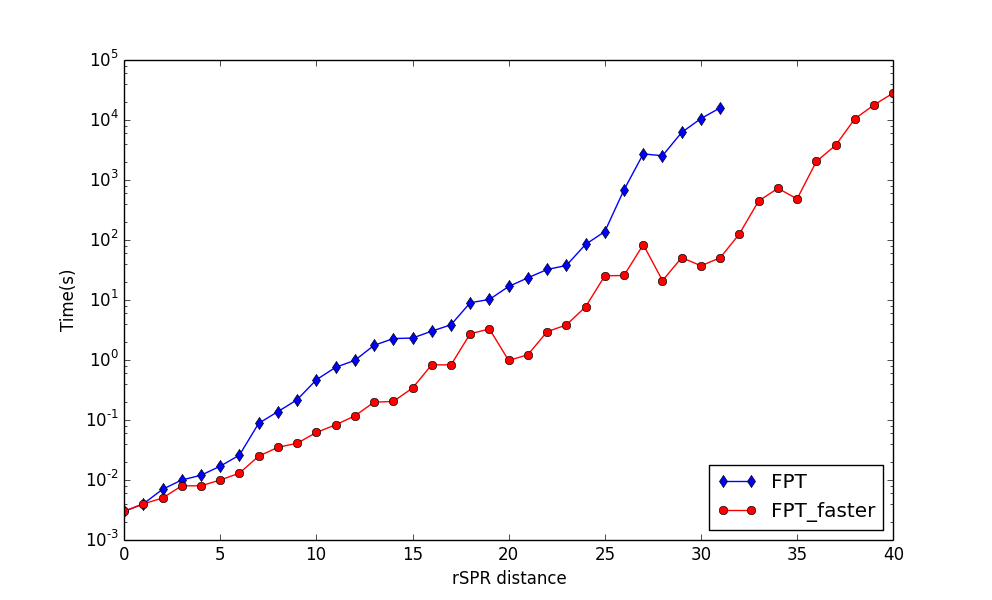
\includegraphics[width=0.9\textwidth, height=0.7\textheight, keepaspectratio]{./pic/figure_1.png}
\end{frame}

\begin{frame}{特殊随机数据测试}
测试了多组经特殊rSPR操作后的进化树对,结果如下:
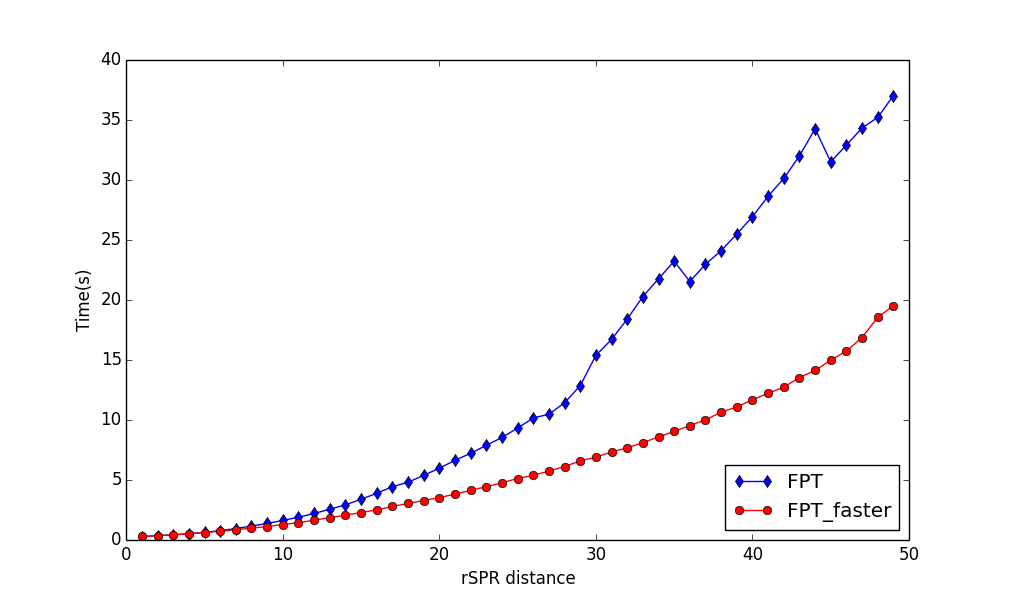
\includegraphics[width=0.9\textwidth, height=0.7\textheight, keepaspectratio]{./pic/figure_3.png}
\end{frame}

\begin{frame}{生物数据测试}
真实的生物数据测试:
\begin{center}
\begin{tabular}{ c c c c }
  \hline
    $d_{rSPR}$ & 组数 & FPT\_faster & FPT  \\ \hline
    0 & 8 & 0.001s & 0.001s  \\
    1 & 12 & 0.002s & 0.002s \\
    2 & 4 & 0.002s & 0.002s  \\
    3 & 7 & 0.003s & 0.003s  \\
    4 & 9 & 0.003s & 0.004s  \\
    5 & 5 & 0.004s & 0.006s  \\
    6 & 2 & 0.005s & 0.007s \\
    7 & 4 & 0.010s & 0.023s \\
    8 & 2 & 0.021s & 0.027s \\
    9 & 1 & 0.013s & 0.022s \\
    12 & 2 & 0.173s & 0.534s \\
    17 & 1 & 3.916s & 21.034s \\
  \hline
\end{tabular}
\end{center}
\end{frame}

\section{致谢}
\begin{frame}
\vspace{2cm}
  \begin{center}
    \huge{最后,感谢各位老师在百忙之中给了我这次提前答辩的机会}
  \end{center}
\end{frame}

\end{document}













